% ============================================================
\chapter{G\'eod\'esiques et Application Exponentielle}
\label{ch:geodesiques}
% ============================================================

Quel est le plus court chemin entre deux points sur une sph\`ere~? Un grand cercle, bien s\^ur. Mais comment formuler cette question sur une vari\'et\'e riemannienne quelconque~? La r\'eponse passe par les \emph{g\'eod\'esiques}~: les courbes qui ne tournent pas, celles dont l'acc\'el\'eration covarienne est nulle. Sur un plan, ce sont les droites~; sur une sph\`ere, les grands cercles~; sur une surface de r\'evolution, des courbes que l'on peut calculer explicitement gr\^ace aux \'equations d'Euler-Lagrange du calcul des variations. L'\emph{application exponentielle}, qui envoie un vecteur tangent sur le point atteint en temps 1 le long de la g\'eod\'esique correspondante, fournit un syst\`eme de coordonn\'ees local centr\'e en chaque point --- les coordonn\'ees normales, o\`u la m\'etrique est euclidienne au premier ordre.

\section{\'Equation des g\'eod\'esiques}

\begin{definition}[G\'eod\'esique]
Soit $(M, g)$ une vari\'et\'e riemannienne munie de sa connexion de Levi-Civita
$\nabla$. Une courbe lisse $\gamma : I \to M$ est une \emph{g\'eod\'esique} si~:
\[
    \nabla_{\dot\gamma}\dot\gamma = 0.
\]
En coordonn\'ees locales $(x^1, \ldots, x^n)$~:
\[
    \ddot\gamma^k(t) + \Gamma^k_{ij}(\gamma(t))\, \dot\gamma^i(t)\, \dot\gamma^j(t) = 0,
    \quad k = 1, \ldots, n.
\]
\end{definition}

\begin{proposition}[Param\'etrisation \`a vitesse constante]
Si $\gamma$ est une g\'eod\'esique, alors $\norm{\dot\gamma(t)}$ est constant. En
particulier, les g\'eod\'esiques sont param\'etr\'ees proportionnellement \`a la longueur
d'arc.
\end{proposition}

\begin{proof}
$\frac{d}{dt}\inner{\dot\gamma}{\dot\gamma} = 2\inner{\nabla_{\dot\gamma}\dot\gamma}{\dot\gamma}
= 0$.
\end{proof}

\begin{theoreme}[Existence et unicit\'e locale]
Pour tout $p \in M$ et $v \in T_pM$, il existe $\varepsilon > 0$ et une unique
g\'eod\'esique $\gamma_v : (-\varepsilon, \varepsilon) \to M$ telle que
$\gamma_v(0) = p$ et $\dot\gamma_v(0) = v$.
\end{theoreme}

\begin{proof}
L'\'equation des g\'eod\'esiques est un syst\`eme d'EDO du second ordre \`a coefficients
lisses. Le th\'eor\`eme de Cauchy--Lipschitz assure l'existence et l'unicit\'e locales.
\end{proof}

\begin{proposition}[Homog\'en\'eit\'e]
Pour tout $\lambda \in \R$ et $v \in T_pM$, on a~:
$\gamma_{\lambda v}(t) = \gamma_v(\lambda t)$
partout o\`u les deux membres sont d\'efinis.
\end{proposition}

\section{Application exponentielle}

\begin{definition}[Application exponentielle]
L'\emph{application exponentielle} en $p \in M$ est l'application~:
\[
    \exp_p : \mathcal{D}_p \subset T_pM \to M, \quad v \mapsto \gamma_v(1),
\]
o\`u $\mathcal{D}_p$ est le domaine maximal de d\'efinition (ouvert \'etoil\'e contenant
$0$) et $\gamma_v$ est la g\'eod\'esique avec $\gamma_v(0) = p$, $\dot\gamma_v(0) = v$.
\end{definition}

\begin{proposition}
L'application $\exp_p$ est lisse et v\'erifie~:
\begin{enumerate}
    \item $\exp_p(0) = p$.
    \item $(d\exp_p)_0 = \operatorname{Id}_{T_pM}$ (via l'identification canonique
          $T_0(T_pM) \cong T_pM$).
    \item $\exp_p(tv) = \gamma_v(t)$ pour tout $t$ dans le domaine.
\end{enumerate}
\end{proposition}

\begin{proof}
Le point (2) se v\'erifie par~: $(d\exp_p)_0(v) = \frac{d}{dt}\Big|_{t=0} \exp_p(tv)
= \frac{d}{dt}\Big|_{t=0} \gamma_v(t) = \dot\gamma_v(0) = v$.
\end{proof}

\begin{corollaire}
Par le th\'eor\`eme d'inversion locale, $\exp_p$ est un diff\'eomorphisme d'un
voisinage de $0$ dans $T_pM$ sur un voisinage de $p$ dans $M$.
\end{corollaire}

% Diagramme de l'application exponentielle
\begin{center}
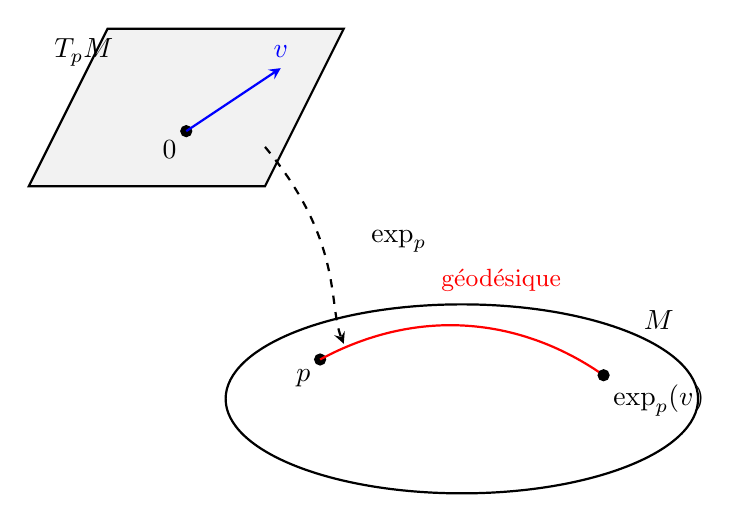
\begin{tikzpicture}[>=stealth, scale=1.0]
  % Plan tangent T_pM (rectangle inclin\'e)
  \fill[gray!10] (-3.5,2.5) -- (-0.5,2.5) -- (0.5,4.5) -- (-2.5,4.5) -- cycle;
  \draw[thick] (-3.5,2.5) -- (-0.5,2.5) -- (0.5,4.5) -- (-2.5,4.5) -- cycle;
  \node at (-2.8,4.2) {$T_pM$};
  % Origine dans le plan tangent
  \filldraw (-1.5,3.2) circle (2pt) node[below left] {$0$};
  % Vecteur v dans le plan tangent
  \draw[->, thick, blue] (-1.5,3.2) -- (-0.3,4.0) node[above] {$v$};
  % Vari\'et\'e M (ellipse en bas)
  \draw[thick] (2,-0.2) ellipse (3cm and 1.2cm);
  \node at (4.5,0.8) {$M$};
  % Point p sur la vari\'et\'e
  \filldraw (0.2,0.3) circle (2pt) node[below left] {$p$};
  % G\'eod\'esique courbe de p \`a exp_p(v)
  \draw[thick, red] (0.2,0.3) .. controls (1.5,1.0) and (2.8,0.8) .. (3.8,0.1);
  \filldraw (3.8,0.1) circle (2pt) node[below right] {$\exp_p(v)$};
  % Fl\`eche exp_p
  \draw[->, thick, dashed] (-0.5,3.0) .. controls (0.5,1.8) and (0.3,1.0) .. (0.5,0.5);
  \node at (1.2,1.8) {$\exp_p$};
  % L\'egende de la g\'eod\'esique
  \node[red] at (2.5,1.3) {\small g\'eod\'esique};
\end{tikzpicture}
\end{center}

\section{Coordonn\'ees normales}

\begin{definition}[Coordonn\'ees normales]
Soit $(e_1, \ldots, e_n)$ une base orthonorm\'ee de $T_pM$. Les \emph{coordonn\'ees
normales} centr\'ees en $p$ sont les coordonn\'ees $x^i$ d\'efinies sur un voisinage
$U$ de $p$ par~:
\[
    q = \exp_p(x^1 e_1 + \cdots + x^n e_n).
\]
\end{definition}

\begin{proposition}[Propri\'et\'es des coordonn\'ees normales]
En coordonn\'ees normales centr\'ees en $p$~:
\begin{enumerate}
    \item $g_{ij}(p) = \delta_{ij}$.
    \item $\Gamma^k_{ij}(p) = 0$.
    \item $\partial_l g_{ij}(p) = 0$.
    \item Les g\'eod\'esiques radiales passant par $p$ sont les droites
          $t \mapsto (tv^1, \ldots, tv^n)$.
    \item Le d\'eveloppement de Taylor de la m\'etrique est~:
          \[
              g_{ij}(x) = \delta_{ij} - \frac{1}{3} R_{ikjl}(p)\, x^k x^l + O(\norm{x}^3).
          \]
\end{enumerate}
\end{proposition}

\begin{proof}
(1) d\'ecoule du choix de base orthonorm\'ee. (2)~: les g\'eod\'esiques radiales
v\'erifient $\gamma(t) = tv$, donc $\ddot\gamma^k = 0$ et l'\'equation des g\'eod\'esiques
donne $\Gamma^k_{ij}(p) v^i v^j = 0$ pour tout $v$, d'o\`u $\Gamma^k_{ij}(p) = 0$
par polarisation. (3) d\'ecoule de (2) et de la formule des Christoffel.
\end{proof}

\begin{intuition}[title=\textbf{Coordonn\'ees normales = lin\'earisation de la g\'eom\'etrie}]
En coordonn\'ees normales, la m\'etrique est euclidienne \`a l'ordre $1$~: les
effets de la courbure n'apparaissent qu'\`a l'ordre $2$. C'est l'analogue
riemannien du fait que la Terre para\^it plate localement.
\end{intuition}

\section{Le lemme de Gauss}

\begin{lemme}[Lemme de Gauss]
\label{lem:gauss}
Soit $p \in M$ et $v \in T_pM$ avec $\exp_p(v)$ d\'efini. Alors~:
\[
    \inner{(d\exp_p)_v(v)}{(d\exp_p)_v(w)} = \inner{v}{w}
\]
pour tout $w \in T_pM$, o\`u on identifie $T_v(T_pM) \cong T_pM$.
\end{lemme}

\begin{proof}
Posons $q = \exp_p(v)$. Le vecteur $(d\exp_p)_v(v) = \dot\gamma_v(1)$ o\`u
$\gamma_v(t) = \exp_p(tv)$. On consid\`ere la variation
$F(t,s) = \exp_p(t(v + sw))$.

Pour $t$ fix\'e, $F(t, \cdot)$ est une courbe de g\'eod\'esiques radiales.
Le champ de Jacobi associ\'e est $J(t) = \frac{\partial F}{\partial s}\big|_{s=0}
= t\, (d\exp_p)_{tv}(w)$.

On calcule~:
\[
    \frac{d}{dt}\inner{\dot\gamma_v(t)}{J(t)}
    = \inner{\underbrace{\nabla_{\dot\gamma}\dot\gamma}_{=0}}{J}
    + \inner{\dot\gamma}{\frac{DJ}{dt}}.
\]
Par sym\'etrie des connexions~:
$\inner{\dot\gamma}{\frac{DJ}{dt}} = \frac{d}{dt}\inner{\dot\gamma}{J}
- \inner{\nabla_{\dot\gamma}\dot\gamma}{J}
= \frac{d}{dt}\inner{\dot\gamma}{J}$.

On montre que $\frac{d}{dt}\inner{\dot\gamma}{J} = \inner{\dot\gamma(0)}{w} = \inner{v}{w}$
en utilisant que $J(0) = 0$ et $\frac{DJ}{dt}(0) = w$. Donc
$\inner{\dot\gamma_v(1)}{J(1)} = \inner{v}{w}$.
Comme $J(1) = (d\exp_p)_v(w)$ et $\dot\gamma_v(1) = (d\exp_p)_v(v)$, le r\'esultat suit.
\end{proof}

\begin{corollaire}[Orthogonalit\'e des sph\`eres g\'eod\'esiques]
Les g\'eod\'esiques radiales issues de $p$ sont orthogonales aux sph\`eres
g\'eod\'esiques $S(p, r) = \{q : d(p,q) = r\}$ (pour $r$ assez petit).
\end{corollaire}

\section{G\'eod\'esiques minimisantes}

\begin{theoreme}[Les g\'eod\'esiques courtes sont minimisantes]
\label{thm:geod_min}
Pour tout $p \in M$, il existe $\varepsilon > 0$ tel que pour tout $q \in B(p, \varepsilon)$,
il existe une unique g\'eod\'esique minimisante de $p$ \`a $q$, et cette g\'eod\'esique
est contenue dans $B(p, \varepsilon)$.
\end{theoreme}

\begin{proof}
On utilise le lemme de Gauss et une comparaison avec les coordonn\'ees normales.
Soit $\gamma$ la g\'eod\'esique radiale de $p$ \`a $q = \exp_p(v)$ et $\sigma : [0,1] \to M$
une courbe quelconque de $p$ \`a $q$. En coordonn\'ees normales, on d\'ecompose
$\dot\sigma = \dot\sigma^r + \dot\sigma^\perp$ en composantes radiale et tangentielle
aux sph\`eres g\'eod\'esiques. Par le lemme de Gauss~:
\[
    L(\sigma) = \int_0^1 \sqrt{|\dot\sigma^r|^2 + |\dot\sigma^\perp|^2}\, dt
    \geq \int_0^1 |\dot\sigma^r|\, dt \geq |r(1) - r(0)| = \norm{v} = L(\gamma).
\]
\end{proof}

\begin{definition}[Voisinage normal]
Un ouvert $U \ni p$ est un \emph{voisinage normal} de $p$ s'il existe un ouvert
\'etoil\'e $V \subset T_pM$ contenant $0$ tel que $\exp_p : V \to U$ est un
diff\'eomorphisme et tout point de $U$ est joint \`a $p$ par une unique g\'eod\'esique
minimisante contenue dans $U$.
\end{definition}

\section{Rayon d'injectivit\'e}

\begin{definition}[Rayon d'injectivit\'e]
Le \emph{rayon d'injectivit\'e} en $p$ est~:
\[
    \operatorname{inj}(p) = \sup\{r > 0 : \exp_p|_{B(0,r)} \text{ est un diff\'eomorphisme}\}.
\]
Le rayon d'injectivit\'e de $M$ est $\operatorname{inj}(M) = \inf_{p \in M} \operatorname{inj}(p)$.
\end{definition}

\begin{exemple}[Rayon d'injectivit\'e de $S^n$]
$\operatorname{inj}(S^n) = \pi$~: l'application exponentielle en tout point cesse
d'\^etre injective au point antipodal.
\end{exemple}

\begin{exemple}[Rayon d'injectivit\'e du tore plat]
Pour $\mathbb{T}^2 = \R^2/\Z^2$, $\operatorname{inj}(\mathbb{T}^2) = 1/2$.
\end{exemple}

\begin{exemple}[Rayon d'injectivit\'e de $\mathbb{H}^n$]
$\operatorname{inj}(\mathbb{H}^n) = +\infty$~: l'application exponentielle est un
diff\'eomorphisme global.
\end{exemple}

\section{Point conjugu\'e et point de coupure}

\begin{definition}[Point conjugu\'e]
Un point $\gamma(t_0)$ est \emph{conjugu\'e} \`a $\gamma(0) = p$ le long de la
g\'eod\'esique $\gamma$ si $(d\exp_p)_{t_0 \dot\gamma(0)}$ est singuli\`ere, i.e.\
s'il existe un champ de Jacobi non nul $J$ le long de $\gamma$ avec
$J(0) = J(t_0) = 0$.
\end{definition}

\begin{definition}[Point de coupure]
Le \emph{point de coupure} de $p$ le long de $\gamma$ est le premier point
$\gamma(t_c)$ au-del\`a duquel $\gamma$ cesse d'\^etre minimisante~:
\[
    t_c = \sup\{t > 0 : \gamma|_{[0,t]} \text{ est minimisante}\}.
\]
Le \emph{lieu de coupure} $\operatorname{Cut}(p)$ est l'ensemble des points de
coupure pour toutes les g\'eod\'esiques issues de $p$.
\end{definition}

\begin{theoreme}[Caract\'erisation du point de coupure]
Le point de coupure $\gamma(t_c)$ v\'erifie l'une des deux conditions~:
\begin{enumerate}
    \item $\gamma(t_c)$ est le premier point conjugu\'e le long de $\gamma$.
    \item Il existe une autre g\'eod\'esique minimisante de $p$ \`a $\gamma(t_c)$.
\end{enumerate}
\end{theoreme}

\begin{exemple}[Lieu de coupure de $S^n$]
Pour $p$ le p\^ole Nord de $S^n$, $\operatorname{Cut}(p) = \{-p\}$ (le point antipodal).
\end{exemple}

\section{G\'eod\'esiques des espaces mod\`eles}

\begin{exemple}[G\'eod\'esiques de $\R^n$]
Les g\'eod\'esiques sont les droites $\gamma(t) = p + tv$.
\end{exemple}

\begin{exemple}[G\'eod\'esiques de $S^n$]
Les g\'eod\'esiques sont les grands cercles, param\'etr\'es par~:
$\gamma(t) = \cos(t)\, p + \sin(t)\, v$,
o\`u $p \in S^n$ et $v \in T_pS^n$ avec $\norm{v} = 1$.
\end{exemple}

\begin{exemple}[G\'eod\'esiques de $\mathbb{H}^2$ (demi-plan)]
Les g\'eod\'esiques sont~:
\begin{itemize}
    \item Les demi-droites verticales $\{x = x_0, y > 0\}$.
    \item Les demi-cercles centr\'es sur l'axe $\{y = 0\}$.
\end{itemize}
Pour une demi-droite verticale param\'etr\'ee par $\gamma(t) = (x_0, e^t)$~:
$\dot\gamma = (0, e^t)$, $\norm{\dot\gamma}_g = \frac{e^t}{e^t} = 1$, et on v\'erifie
que l'\'equation des g\'eod\'esiques est satisfaite.
\end{exemple}

\section{Fonctionnelle d'\'energie et variation premi\`ere}

\begin{definition}[Fonctionnelle d'\'energie]
L'\emph{\'energie} d'une courbe $\gamma : [a,b] \to M$ est~:
\[
    E(\gamma) = \frac{1}{2}\int_a^b \norm{\dot\gamma(t)}^2\, dt.
\]
\end{definition}

\begin{proposition}[In\'egalit\'e de Cauchy--Schwarz]
$L(\gamma)^2 \leq 2(b-a)\, E(\gamma)$, avec \'egalit\'e si et seulement si
$\norm{\dot\gamma}$ est constant.
\end{proposition}

\begin{theoreme}[Formule de la premi\`ere variation]
Soit $\gamma_s : [a,b] \to M$ une variation lisse de $\gamma_0 = \gamma$ avec
champ de variation $V = \frac{\partial\gamma_s}{\partial s}\big|_{s=0}$. Alors~:
\[
    \frac{d}{ds}\bigg|_{s=0} E(\gamma_s) = -\int_a^b \inner{\nabla_{\dot\gamma}\dot\gamma}{V}\, dt
    + \inner{\dot\gamma(b)}{V(b)} - \inner{\dot\gamma(a)}{V(a)}.
\]
\end{theoreme}

\begin{corollaire}
Les points critiques de $E$ parmi les courbes \`a extr\'emit\'es fixes sont exactement
les g\'eod\'esiques. Les g\'eod\'esiques sont donc les \emph{courbes critiques}
de la fonctionnelle d'\'energie (et de longueur).
\end{corollaire}

\section{Compl\'etude g\'eod\'esique et th\'eor\`eme de Hopf--Rinow}

\begin{definition}
$(M, g)$ est \emph{g\'eod\'esiquement compl\`ete} si toute g\'eod\'esique peut \^etre
prolong\'ee pour tout temps $t \in \R$.
\end{definition}

Nous rappelons que le th\'eor\`eme de Hopf--Rinow (Th\'eor\`eme~\ref{thm:hopf_rinow})
montre l'\'equivalence entre compl\'etude m\'etrique et compl\'etude g\'eod\'esique.

\section{Exercices}

\begin{exercice}
Calculer les g\'eod\'esiques du cylindre $S^1 \times \R$ muni de la m\'etrique produit.
Montrer que ce sont des h\'elices (y compris les cercles et les droites comme cas
limites).
\end{exercice}

\begin{exercice}
Montrer que les g\'eod\'esiques de $\mathbb{H}^2$ dans le mod\`ele du disque de
Poincar\'e sont les diam\`etres et les arcs de cercle orthogonaux au bord $\partial\mathbb{D}$.
\end{exercice}

\begin{exercice}
Soit $G = SU(2)$ muni de la m\'etrique bi-invariante. Identifier $SU(2) \cong S^3$
et montrer que les g\'eod\'esiques sont les grands cercles.
\end{exercice}

\begin{exercice}
Calculer le rayon d'injectivit\'e du plan projectif r\'eel $\R P^n$ muni de la
m\'etrique quotient de $S^n$.
\end{exercice}

\begin{exercice}
Montrer que sur une surface de r\'evolution $g = du^2 + f(u)^2 dv^2$, les
g\'eod\'esiques v\'erifient la loi de Clairaut~: $f(u(\gamma))^2\, \dot v(\gamma) = c$
(constante le long de la g\'eod\'esique).
\end{exercice}

\begin{exercice}
D\'emontrer la formule de la premi\`ere variation de la longueur~: si $\gamma$ est
param\'etr\'ee par longueur d'arc~:
\[
    \frac{d}{ds}\bigg|_{s=0} L(\gamma_s)
    = -\int_a^b \inner{\nabla_{\dot\gamma}\dot\gamma}{V}\, dt
    + \inner{\dot\gamma}{V}\Big|_a^b.
\]
\end{exercice}
